% Gabarit pandoc des corrigés publiés (brut et guidé). Contenu sans marque ni nom de site.
% Compilation : lualatex (latexmk -lualatex).
% Le Markdown reste la source unique : ne pas éditer ce fichier .tex à la main.
\documentclass[11pt,a4paper]{article}

% --- Moteur, polices (Latin Modern) et langue ---------------------------------
\usepackage{iftex}
\ifLuaTeX\else\errmessage{Ce document se compile avec lualatex}\fi
\usepackage{amsmath,amssymb,mathtools}
\usepackage{fontspec}
% mathrm=sym : \mathrm prend ses glyphes dans la police mathématique (ℓ, μ, Ω), comme KaTeX.
\usepackage[math-style=TeX,bold-style=TeX,mathrm=sym]{unicode-math}
% Repli pour les glyphes absents de Latin Modern (indices et exposants Unicode,
% flèches, filets des schémas en texte, symboles) : DejaVu, puis Latin Modern Math
% (ℓ, lettres mathématiques Unicode des légendes).
\directlua{
  luaotfload.add_fallback("repliTexte", {"DejaVuSerif:mode=harf;", "DejaVuSans:mode=harf;", "file:latinmodern-math.otf:mode=harf;"})
  luaotfload.add_fallback("repliMono", {"DejaVuSansMono:mode=harf;", "DejaVuSans:mode=harf;", "file:latinmodern-math.otf:mode=harf;"})
}
\setmainfont{Latin Modern Roman}[RawFeature={fallback=repliTexte}]
\setsansfont{Latin Modern Sans}[RawFeature={fallback=repliTexte}]
\setmonofont{Latin Modern Mono}[RawFeature={fallback=repliMono}]
\setmathfont{Latin Modern Math}
\usepackage[french]{babel}
\frenchsetup{SmallCapsFigTabCaptions=false}

% --- Mise en page --------------------------------------------------------------
\usepackage[a4paper,margin=2.2cm,headheight=14pt,footskip=1.2cm]{geometry}
\usepackage{microtype}
\setlength{\emergencystretch}{4em}
\tolerance=1500
\setlength{\parindent}{0pt}
\setlength{\parskip}{0.55\baselineskip plus 2pt minus 1pt}
\usepackage{xcolor}
% Gris nommés : babel-french rend « ! » actif dans le document.
\definecolor{gris2}{gray}{0.98}
\definecolor{gris3}{gray}{0.97}
\definecolor{gris5}{gray}{0.95}
\definecolor{gris35}{gray}{0.65}
\definecolor{gris40}{gray}{0.60}
\definecolor{gris45}{gray}{0.55}
\definecolor{gris50}{gray}{0.50}
\definecolor{gris55}{gray}{0.45}
\definecolor{gris60}{gray}{0.40}
\definecolor{gris65}{gray}{0.35}
\definecolor{gris70}{gray}{0.30}
\definecolor{gris80}{gray}{0.20}
\definecolor{gris85}{gray}{0.15}
\usepackage{graphicx}
\usepackage{float}
\usepackage{caption}
\captionsetup{font=small,labelformat=empty,justification=centering}
\usepackage{booktabs,longtable,array,multirow,calc}
\usepackage{siunitx}
\sisetup{locale=FR}
\usepackage[version=4]{mhchem}
\usepackage{listings}
\usepackage{fancyhdr}
\usepackage{lastpage}
\usepackage[most]{tcolorbox}
\usepackage{enumitem}
\setlist{nosep,leftmargin=*,topsep=2pt}
\usepackage[hidelinks,unicode]{hyperref}
\usepackage{bookmark}
\hypersetup{pdftitle={X-ENS MP — Informatique A 2026},pdfauthor={Rédigé par IA},pdfcreator={LaTeX},pdfsubject={Corrigé brut}}
\usepackage{xurl}

% --- Pandoc : listes, tableaux, figures ----------------------------------------
\providecommand{\passthrough}[1]{#1}
\providecommand{\tightlist}{\setlength{\itemsep}{0pt}\setlength{\parskip}{0pt}}

\makeatletter
\def\maxwidth{\ifdim\Gin@nat@width>\linewidth\linewidth\else\Gin@nat@width\fi}
\def\maxheight{\ifdim\Gin@nat@height>0.55\textheight 0.55\textheight\else\Gin@nat@height\fi}
\makeatother
\setkeys{Gin}{width=\maxwidth,height=\maxheight,keepaspectratio}
\setcounter{secnumdepth}{-\maxdimen}
\providecommand{\pandocbounded}[1]{#1}

% --- Code (listings) -----------------------------------------------------------
\lstset{
  basicstyle=\ttfamily\small,
  columns=fullflexible,
  keepspaces=true,
  breaklines=true,
  breakatwhitespace=false,
  postbreak=\mbox{\textcolor{gris50}{$\hookrightarrow$}\space},
  frame=single,
  rulecolor=\color{gris35},
  framesep=4pt,
  xleftmargin=5pt,xrightmargin=5pt,
  backgroundcolor=\color{gris3},
  keywordstyle=\bfseries,
  commentstyle=\color{gris65},
  stringstyle=\color{gris80},
  showstringspaces=false,
  tabsize=4,
  extendedchars=true,
  aboveskip=6pt,belowskip=6pt,
}

% --- Macros des corrigés (KaTeX ↔ LaTeX) ---------------------------------------
% Les corrigés sont écrits pour KaTeX : on définit ici ce que KaTeX connaît et
% que LaTeX n'a pas, sans jamais retoucher le Markdown.
\providecommand{\R}{\mathbb{R}}
\providecommand{\N}{\mathbb{N}}
\providecommand{\Z}{\mathbb{Z}}
\providecommand{\Q}{\mathbb{Q}}
\providecommand{\C}{\mathbb{C}}
\providecommand{\dd}{\mathrm{d}}
\providecommand{\llbracket}{\lBrack}
\providecommand{\rrbracket}{\rBrack}
\providecommand{\lBrace}{\lbrace}
\providecommand{\rBrace}{\rbrace}
\providecommand{\Box}{\square}
\providecommand{\Diamond}{\lozenge}
\providecommand{\varnothing}{\emptyset}
\providecommand{\argmax}{\operatorname*{arg\,max}}
\providecommand{\argmin}{\operatorname*{arg\,min}}
\renewcommand{\leq}{\leqslant}
\renewcommand{\geq}{\geqslant}

% Équation hors texte : réduite à la largeur de la ligne si elle déborde.
\newsavebox{\boiteequation}
\newcommand{\equationajustee}[1]{%
  \sbox{\boiteequation}{$\displaystyle #1$}%
  \ifdim\wd\boiteequation>\linewidth
    \[\resizebox{\linewidth}{!}{\usebox{\boiteequation}}\]%
  \else
    \[#1\]%
  \fi}

% --- Encadrés pédagogiques (sobres, lisibles en noir et blanc) -----------------
\tcbset{
  encadre/.style={
    enhanced,breakable,sharp corners,
    colback=white,colframe=gris55,
    boxrule=0.4pt,leftrule=2.2pt,
    left=6pt,right=6pt,top=3pt,bottom=3pt,
    before skip=6pt,after skip=6pt,
    fonttitle=\bfseries\small,coltitle=black,
    attach title to upper,after title={\quad},
    parbox=false,
  }
}
\newtcolorbox{indication}[1]{encadre,colframe=gris45,colback=gris2,title={Indication~#1}}
\newtcolorbox{methode}{encadre,colframe=gris70,title={Méthode}}
\newtcolorbox{piege}{encadre,colframe=gris85,boxrule=0.8pt,leftrule=2.2pt,title={Piège}}
\newtcolorbox{jury}{encadre,colframe=gris60,colback=gris5,title={Jury}}
\newtcolorbox{encadrenote}{encadre,colframe=gris40}

% --- Titres de section ---------------------------------------------------------
\usepackage{titlesec}
\titleformat{\section}{\Large\bfseries}{}{0pt}{}
\titleformat{\subsection}{\large\bfseries}{}{0pt}{}
\titleformat{\subsubsection}{\normalsize\bfseries}{}{0pt}{}
\titlespacing*{\section}{0pt}{14pt plus 4pt minus 2pt}{6pt}
\titlespacing*{\subsection}{0pt}{10pt plus 3pt minus 2pt}{4pt}
\titlespacing*{\subsubsection}{0pt}{8pt plus 2pt minus 2pt}{2pt}

% --- En-tête et pied de page ---------------------------------------------------
\pagestyle{fancy}
\fancyhf{}
\fancyhead[L]{\small\textsc{Corrigé brut} · X-ENS MP}
\fancyhead[R]{\small Informatique A 2026}
\fancyfoot[L]{\footnotesize Corrigé rédigé par IA, non officiel}
\fancyfoot[R]{\footnotesize \thepage\,/\,\pageref*{LastPage}}
\renewcommand{\headrulewidth}{0.4pt}
\renewcommand{\footrulewidth}{0pt}
\fancypagestyle{plain}{\fancyhf{}\fancyfoot[R]{\footnotesize \thepage\,/\,\pageref*{LastPage}}\fancyfoot[L]{\footnotesize Corrigé rédigé par IA, non officiel}\renewcommand{\headrulewidth}{0pt}}

\begin{document}
\thispagestyle{plain}
\begin{center}
  {\small\scshape Corrigé brut}\par\smallskip
  {\LARGE\bfseries X-ENS MP — Informatique A 2026\par}\medskip
  {\large X-ENS · MP · Informatique A · 2026\par}
\end{center}
\vspace{2pt}\hrule\vspace{8pt}

\emph{Corrigé rédigé par IA, non officiel. Signalez toute erreur.}

\emph{Bases de données de vecteurs.} Durée 4 h, calculatrice interdite, langage OCaml. On note \([n]=\{0,\dots,n-1\}\) et \(\log\) le logarithme en base 2.

\begin{center}\rule{0.5\linewidth}{0.5pt}\end{center}

\hypertarget{partie-i.-reconnaissance-automatique-dextraits-musicaux}{%
\section{Partie I. Reconnaissance automatique d'extraits musicaux}\label{partie-i.-reconnaissance-automatique-dextraits-musicaux}}

\hypertarget{question-i.1}{%
\subsection{Question I.1}\label{question-i.1}}

Le spectrogramme se lit comme un mot : chaque instant \(t\) est une « lettre », la colonne de hauteur \(F\), prise dans l'alphabet \(\{\texttt{' '},\texttt{'x'}\}^F\).

Chercher si une musique de durée \(D\) est exactement un extrait d'une musique de durée \(T\), c'est chercher une occurrence d'un motif (l'extrait) dans un texte (la musique). C'est le problème de \textbf{recherche de motif dans un texte} (\emph{pattern matching}).

Recherche naïve : pour chaque position de départ \(t\in\{0,\dots,T-D\}\), il y en a \(T-D+1\), on compare l'extrait à la fenêtre des colonnes \(t,\dots,t+D-1\), colonne par colonne et case par case, en s'arrêtant au premier désaccord. Une comparaison examine au plus \(F\cdot D\) cases. Ce maximum est atteint à chaque position, par exemple si toutes les colonnes du texte et de l'extrait sont identiques sauf la dernière colonne de l'extrait. Le pire cas coûte donc

\equationajustee{\boxed{O\big(F\cdot D\cdot(T-D+1)\big)},}

c'est-à-dire \(O(D\,T\,F)\), puisque \(T-D+1\le T\).

\hypertarget{question-i.2}{%
\subsection{Question I.2}\label{question-i.2}}

\begin{lstlisting}[language=Caml]
let to_sparse (s : spectrogram) : sparse =
  let res = ref [] in
  for f = Array.length s - 1 downto 0 do
    for t = Array.length s.(f) - 1 downto 0 do
      if s.(f).(t) = 'x' then res := (f, t) :: !res
    done
  done;
  !res
\end{lstlisting}

On parcourt les cases de la dernière à la première et on ajoute en tête. La liste obtenue contient exactement les \((f,t)\) tels que \texttt{s.(f).(t)\ =\ \textquotesingle{}x\textquotesingle{}}, triés dans l'ordre lexicographique croissant. Le coût est \(O(F\,T)\).

\hypertarget{question-i.3}{%
\subsection{Question I.3}\label{question-i.3}}

\begin{lstlisting}[language=Caml]
let convert (l : int list) : int =
  List.fold_left (fun acc i -> acc lor (1 lsl i)) 0 l
\end{lstlisting}

\texttt{1\ lsl\ i} est l'entier dont seul le bit \(i\) vaut 1, et le « ou » bit à bit accumule ces bits. Comme la liste est sans doublons, on peut aussi écrire \texttt{acc\ +\ (1\ lsl\ i)} : les bits ajoutés sont distincts, donc il n'y a jamais de retenue. Coût : \(O(|l|)\).

\hypertarget{question-i.4}{%
\subsection{Question I.4}\label{question-i.4}}

\begin{lstlisting}[language=Caml]
let inter (a : int) (b : int) : int = a land b
\end{lstlisting}

Le bit \(i\) de \texttt{a\ land\ b} vaut 1 si et seulement si le bit \(i\) de \texttt{a} et celui de \texttt{b} valent tous deux 1, c'est-à-dire si \(i\) appartient aux deux sous-ensembles. Coût \(O(1)\).

\hypertarget{question-i.5}{%
\subsection{Question I.5}\label{question-i.5}}

\textbf{(a)}

\begin{lstlisting}[language=Caml]
let size (n : int) : int =
  let count = ref 0 in
  let b = ref n in
  while !b <> 0 do
    b := !b - (!b land (- !b));
    count := !count + 1
  done;
  !count
\end{lstlisting}

D'après l'indication, \texttt{!b\ land\ (-\ !b)} vaut \(2^j\), où \(j\) est l'indice du bit à 1 de poids le plus faible de \texttt{!b}. Ce bit valant 1, la soustraction le met à 0 sans retenue et laisse les autres bits inchangés. Chaque tour de boucle éteint donc exactement un bit.

Soit \(s\) le cardinal de l'ensemble codé par \(n\). On fait exactement \(s\) tours, chacun de coût \(O(1)\). La complexité est donc \(\boxed{O(s)}\), linéaire en la taille de l'ensemble.

\textbf{(b)} Pour un entier \(x\geq 0\), on note \(\mathrm{pc}(x)\) le nombre de bits à 1 de \(x\). On pose \(s=\mathrm{pc}(n)\).

Comme \(n\) code une partie de \([62]\), on a \(n\geq0\).

\emph{Invariant} (vrai à chaque test de la boucle) : \(\texttt{!b}\geq 0\) et \(\texttt{!count}+\mathrm{pc}(\texttt{!b})=s\).

\begin{itemize}
\tightlist
\item
  \emph{Initialisation} : \(\texttt{!count}=0\) et \(\texttt{!b}=n\), donc \(0+\mathrm{pc}(n)=s\).
\item
  \emph{Conservation} : si \(\texttt{!b}\neq0\), le tour éteint exactement un bit. Alors \(\mathrm{pc}(\texttt{!b})\) diminue de 1, \texttt{!count} augmente de 1, et \texttt{!b} reste positif.
\item
  \emph{Terminaison} : \texttt{!b} est un entier positif qui décroît strictement à chaque tour, c'est un variant. La boucle s'arrête donc, et elle s'arrête avec \(\texttt{!b}=0\).
\item
  \emph{Conclusion} : à la sortie, \(\mathrm{pc}(0)=0\), donc \(\texttt{!count}=s\). La fonction renvoie bien le cardinal.
\end{itemize}

\hypertarget{question-i.6}{%
\subsection{Question I.6}\label{question-i.6}}

\textbf{(a)}

\begin{lstlisting}[language=Caml]
let rec sparse_inter (a : 'a list) (b : 'a list) : int =
  match a, b with
  | [], _ | _, [] -> 0
  | x :: a', y :: b' ->
      if x = y then 1 + sparse_inter a' b'
      else if x < y then sparse_inter a' b
      else sparse_inter a b'
\end{lstlisting}

Les comparaisons \texttt{=} et \texttt{\textless{}} sont polymorphes : la fonction convient aux entiers comme aux \(d\)-uplets. Elle est correcte grâce au tri strictement croissant.

Si \(x<y\), alors \(x\) est plus petit que tous les éléments de \(b\), donc \(x\notin b\) et on peut l'écarter. Le cas \(x>y\) est symétrique. Si \(x=y\), c'est un élément commun, et il n'apparaît plus ensuite puisque les listes sont sans répétition.

\textbf{(b)} Chaque appel récursif retire au moins une tête, une ou deux. Le nombre d'appels est donc au plus \(|a|+|b|+1\), et chaque appel fait un nombre borné de comparaisons en \(O(1)\). La complexité est \(\boxed{O(|a|+|b|)}\).

\hypertarget{question-i.7}{%
\subsection{Question I.7}\label{question-i.7}}

\textbf{(a)}

\begin{lstlisting}[language=Caml]
let tosignature (sp : sparse) (delta : int) : signature =
  let a = Array.of_list sp in
  let n = Array.length a in
  let res = ref [] in
  for i = 0 to n - 1 do
    let (f1, t1) = a.(i) in
    for j = 0 to n - 1 do
      let (f2, t2) = a.(j) in
      let d = t2 - t1 in
      if 0 < d && d <= delta then res := (f1, f2, d) :: !res
    done
  done;
  !res
\end{lstlisting}

Un triplet \((f_1,f_2,\delta)\) est ajouté si et seulement s'il existe deux occurrences \((f_1,t)\) et \((f_2,t+\delta)\) dont l'écart vérifie

\equationajustee{0<\delta\le\Delta.}

C'est exactement la définition (1). Si le même triplet est réalisé à plusieurs instants \(t\), il figure plusieurs fois dans la liste. Le supprimer en double ferait perdre la borne \(O(n^2)\), et la question I.8 compte précisément les couples d'occurrences.

\textbf{(b)} \texttt{Array.of\_list} coûte \(O(n)\). Les deux boucles imbriquées font \(n^2\) tours, chacun en \(O(1)\) : accès au tableau, test, ajout en tête. Le total est \(\boxed{O(n^2)}\).

\hypertarget{question-i.8}{%
\subsection{Question I.8}\label{question-i.8}}

\textbf{(a)}

\begin{lstlisting}[language=Caml]
let signature_size (sp : sparse) (delta : int) : int =
  let q = Queue.create () in
  let count = ref 0 in
  List.iter (fun (_, t) ->
      while Queue.length q > 0 && t - Queue.peek q > delta do
        Queue.drop q
      done;
      count := !count + Queue.length q;
      Queue.push t q)
    sp;
  !count
\end{lstlisting}

Sur les exemples : avec \texttt{{[}(1,1);\ (5,5){]}} et \(\Delta=3\), on obtient 0. Avec les cinq couples et \(\Delta=10\), on obtient \(0+1+2+3+4=10\).

\textbf{(b)} \emph{Correction.} La liste \texttt{sp} est triée par temps croissant, et les temps sont distincts. Pour \(i<j\), on a donc \(t_j-t_i>0\). Le couple d'occurrences \((i,j)\) fournit alors un triplet si et seulement si \(t_j-t_i\le\Delta\).

Invariant : juste avant le traitement de \(t_j\), la file contient, dans l'ordre croissant, les \(t_i\) (\(i<j\)) tels que \(t_{j-1}-t_i\le\Delta\).

\begin{itemize}
\tightlist
\item
  À l'arrivée de \(t_j\), la boucle \texttt{while} retire de la tête les temps \(t_i\) tels que \(t_j-t_i>\Delta\). La file est croissante, donc ces temps forment un préfixe. Si \(t_j-t_i>\Delta\), alors \(t_{j'}-t_i>\Delta\) pour tout \(j'>j\) : un temps retiré ne pourra plus jamais servir.
\item
  La file contient alors exactement les partenaires valides de \(t_j\). On ajoute leur nombre au compteur, puis on enfile \(t_j\), ce qui rétablit l'invariant.
\end{itemize}

\begin{figure}[H]
\centering
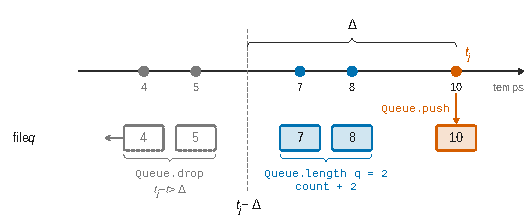
\includegraphics{figures/i8-file-fenetre-glissante.pdf}
\caption*{Figure 1 --- Un pas de signature\_size avec Δ = 4 : à l'arrivée de t\_j
= 10, les instants 4 et 5 sont défilés, les deux instants restants
donnent 2 triplets, puis t\_j est enfilé}
\end{figure}

En sommant sur \(j\), on obtient le nombre de triplets, c'est-à-dire \(|S_\Delta(M)|\).

\emph{Complexité.} La liste est parcourue une seule fois. Chaque temps est enfilé une fois et défilé au plus une fois : la boucle \texttt{while} fait donc au plus \(n\) tours \textbf{au total} sur tout le parcours, et non \(n\) tours par élément.

Toutes les opérations de file, \texttt{Queue.length} comprise, sont en \(O(1)\) d'après l'énoncé. La complexité est amortie linéaire : \(\boxed{O(n)}\).

\hypertarget{question-i.9}{%
\subsection{Question I.9}\label{question-i.9}}

\textbf{C'est la musique \(A\).} Les deux musiques partagent chacune trois triplets avec \(M\) : l'indice de Jaccard ne les départage pas, il faut regarder les temps.

Pour \(A\), l'histogramme des écarts \(t'^{(A)}_i-t_i\) est concentré sur une seule valeur : les trois écarts valent environ 1. Les triplets communs apparaissent donc dans \(A\) avec un \textbf{même décalage temporel}, ce qui veut dire que \(M\) est un morceau de \(A\) translaté dans le temps.

Ce qui compte est cette concentration, et non la petitesse de l'écart : un décalage commun de 100 serait tout aussi probant, l'extrait commençant alors plus loin dans le morceau.

Pour \(B\), les écarts sont dispersés, vers 3, 8 et 11 environ. Aucun décalage commun n'explique les correspondances, qui sont donc fortuites, par exemple dues à du bruit.

\hypertarget{question-i.10}{%
\subsection{Question I.10}\label{question-i.10}}

\textbf{(a)} Soient \(A,B\subset E\) non vides. La numérotation \(h\) est une permutation, donc ses valeurs sont distinctes. Soit \(x^\star\) l'unique élément de \(A\cup B\) qui minimise \(h\). Montrons que
\equationajustee{\mathsf{minHash}(h)(A)=\mathsf{minHash}(h)(B)\iff x^\star\in A\cap B.}

\begin{itemize}
\item
  Si \(x^\star\in A\cap B\) : \(x^\star\) minimise \(h\) sur \(A\cup B\) et appartient aux deux ensembles, donc

  \equationajustee{\min_A h=h(x^\star)=\min_B h.}
\item
  Si \(x^\star\notin A\cap B\), par exemple \(x^\star\in A\setminus B\), alors \(\min_A h=h(x^\star)\).

  Le minimum de \(h\) sur \(B\) est atteint en un élément \(b\neq x^\star\), puisque \(x^\star\notin B\).
  Comme \(h\) est injective et \(b\in A\cup B\), on a \(h(b)>h(x^\star)\) : les deux minima diffèrent.
\end{itemize}

La permutation \(h\) est uniforme : chaque élément de \(A\cup B\) a la même probabilité de porter le plus petit numéro. Ainsi \(x^\star\) suit la loi uniforme sur \(A\cup B\), d'où

\equationajustee{\boxed{\begin{aligned}
\Pr\big(\mathsf{minHash}(h)(A)=\mathsf{minHash}(h)(B)\big)&=\Pr(x^\star\in A\cap B)\\
&=\frac{|A\cap B|}{|A\cup B|}\\
&=J(A,B).
\end{aligned}}}

\textbf{(b)} Méthode.

\begin{enumerate}
\def\labelenumi{\arabic{enumi}.}
\tightlist
\item
  \emph{Prétraitement de la base.} Pour chaque musique \(X\), on calcule sa représentation concise (I.2), puis sa signature \(S_\Delta(X)\) (I.7). On tire \(r\) fonctions de hachage indépendantes \(h_1,\dots,h_r\), et on stocke seulement le vecteur \(\sigma(X)=\big(\mathsf{minHash}(h_1)(S_\Delta(X)),\allowbreak \dots,\allowbreak \mathsf{minHash}(h_r)(S_\Delta(X))\big)\in[N]^r\). Sa taille est fixe, quelle que soit la taille de \(S_\Delta(X)\), ce qui fait gagner de la mémoire.
\item
  \emph{Requête.} On calcule de même \(\sigma(M)\) pour l'extrait \(M\). Pour chaque musique \(X\), on mesure la proportion de coordonnées où \(\sigma(M)\) et \(\sigma(X)\) coïncident.
  D'après (a), c'est une moyenne de \(r\) variables de Bernoulli indépendantes, de paramètre \(J(S_\Delta(M),S_\Delta(X))\). C'est donc un estimateur sans biais de l'indice de Jaccard, de variance au plus \(1/(4r)\).
\item
  On renvoie les musiques qui ont la plus grande similarité estimée. On peut ensuite départager les meilleures candidates par le critère de cohérence temporelle de I.9 : on garde celle dont les écarts \(t'-t\) des triplets communs sont concentrés sur une seule valeur.
\end{enumerate}

Pour éviter de comparer l'extrait à toute la base, on peut ranger les musiques dans des tables indexées par des blocs de coordonnées de \(\sigma\). On ne compare alors l'extrait qu'aux musiques qui partagent au moins un bloc avec lui.

\begin{center}\rule{0.5\linewidth}{0.5pt}\end{center}

\hypertarget{partie-ii.-listes-uxe0-sauts-et-graphes-hiuxe9rarchiques-navigables}{%
\section{Partie II. Listes à sauts et graphes hiérarchiques navigables}\label{partie-ii.-listes-uxe0-sauts-et-graphes-hiuxe9rarchiques-navigables}}

\hypertarget{question-ii.1}{%
\subsection{Question II.1}\label{question-ii.1}}

\begin{lstlisting}[language=Caml]
let skip_length (skl : skip_list) : int =
  let rec aux node acc =
    match node.successors.(0) with
    | None -> acc
    | Some next -> aux next (acc + 1)
  in
  aux skl.init_node 0
\end{lstlisting}

L'étage 0 est la liste chaînée triée de toutes les valeurs. On part du nœud factice, que l'on ne compte pas, et chaque successeur rencontré compte pour une valeur. Coût : \(O(n)\).

\hypertarget{question-ii.2}{%
\subsection{Question II.2}\label{question-ii.2}}

Une valeur \(v\) insérée est présente aux étages \(0,\dots,\ell_v\), où \(\ell_v\) est le niveau renvoyé par \texttt{random\_level}.

Les étages n'étant pas bornés, on a \(\ell_v\geq\ell\) si et seulement si les \(\ell\) premiers tirages \texttt{Random.float\ 1.\ \textless{}\ p} réussissent. Ces tirages sont indépendants et chacun réussit avec probabilité \(p\), donc

\equationajustee{\Pr(\ell_v\geq\ell)=p^\ell.}

On note \(X_v\) l'indicatrice de l'événement « \(v\) est présente à l'étage \(\ell\) ». Par linéarité de l'espérance, le nombre moyen de valeurs présentes à l'étage \(\ell\) est

\equationajustee{\boxed{\mathbb E\Big[\sum_v X_v\Big]=n\,p^{\ell}.}}

\hypertarget{question-ii.3}{%
\subsection{Question II.3}\label{question-ii.3}}

\textbf{(a)}

\begin{lstlisting}[language=Caml]
let search (skl : skip_list) (v : int) : skip_node option =
  let rec descend node level =
    match node.successors.(level) with
    | Some nx when nx.value = v -> Some nx
    | Some nx when nx.value < v -> descend nx level
    | _ -> if level = 0 then None else descend node (level - 1)
  in
  descend skl.init_node skl.init_level
\end{lstlisting}

\textbf{(b)} \emph{Invariant} de chaque appel \texttt{descend\ node\ level} : \texttt{node.value} \(<v\) (le nœud factice vaut \(0<v\)), et \texttt{node} est présent à l'étage \texttt{level}. Le premier point vient de ce qu'on n'avance que vers des valeurs \(<v\).

\emph{Terminaison.} Le couple (\texttt{level}, nombre de nœuds de l'étage 0 situés après \texttt{node}) décroît strictement pour l'ordre lexicographique à chaque appel. Quand on avance, le niveau reste le même et le nœud recule d'au moins un rang. Quand on descend, le niveau diminue.

\emph{Correction.} Si la fonction renvoie \texttt{Some\ nx}, alors \texttt{nx.value} \(=v\). Si elle renvoie \texttt{None}, c'est qu'on est à l'étage 0 et que le successeur de \texttt{node} est absent ou porte une valeur \(>v\). L'étage 0 est la liste triée de toutes les valeurs et \texttt{node.value} \(<v\), donc aucune valeur égale à \(v\) n'existe : \(v\) est absente.

\textbf{(c)} Le nœud courant ne recule jamais dans l'ordre de l'étage 0. Il y a donc au plus \(n\) avancées, et au plus \(\texttt{init\_level}+1\le L\) descentes. La complexité dans le pire cas est \(\boxed{O(n+L)}\).

Elle est atteinte, par exemple, quand la plus petite valeur est présente jusqu'à l'étage \(L-1\) et que toutes les autres sont restées à l'étage 0. Pour chercher la plus grande valeur, on avance jusqu'à la plus petite, on descend les \(L-1\) étages, puis on parcourt les \(n-1\) autres valeurs à l'étage 0.

\hypertarget{question-ii.4}{%
\subsection{Question II.4}\label{question-ii.4}}

On parcourt le chemin à l'envers. Soit \((x,i)\) une position du chemin inversé qui n'est pas encore à l'étage visé. Dans le sens direct, on est arrivé en \((x,i)\) de l'une des deux façons suivantes :

\begin{itemize}
\tightlist
\item
  en \textbf{descendant} depuis \((x,i+1)\), si \(x\) est présent à l'étage \(i+1\). À l'envers, on monte d'un étage ;
\item
  \textbf{horizontalement} depuis le prédécesseur de \(x\) à l'étage \(i\), sinon. À l'envers, on reste à l'étage \(i\).
\end{itemize}

En effet, si \(x\) est présent à l'étage \(i+1\), la recherche directe l'y a atteint, puis elle a dû y descendre, car son successeur à cet étage est absent ou de valeur \(\geq v\).

Sachant que \(x\) est présent à l'étage \(i\), il l'est aussi à l'étage supérieur avec probabilité \(p\) : \texttt{random\_level} fait un tirage indépendant de plus. Ce tirage est indépendant de la partie du chemin déjà remontée.

\begin{figure}[H]
\centering
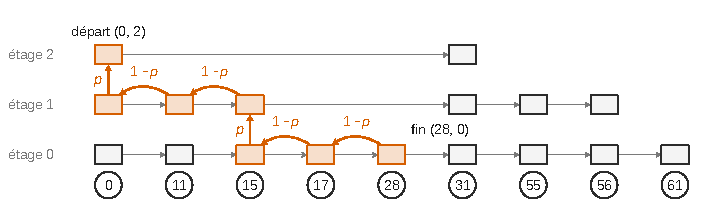
\includegraphics{figures/ii4-chemin-inverse-skip-list.pdf}
\caption*{Figure 2 --- Chemin de recherche de 28 dans la skip list de la figure 3
du sujet, lu à l'envers : montée avec probabilité p, recul au même étage
avec probabilité 1 − p}
\end{figure}

On note \(C_\ell\) le nombre moyen de pas pour monter de \(\ell\) étages. Un pas coûte 1. Avec probabilité \(p\), il reste \(\ell-1\) étages à monter ; avec probabilité \(1-p\), il en reste toujours \(\ell\). D'où

\equationajustee{C_0=0}

et, pour \(\ell\geq1\),

\equationajustee{\begin{aligned}
C_\ell&=1+p\,C_{\ell-1}+(1-p)\,C_\ell\\
p\,C_\ell&=1+p\,C_{\ell-1}\\
C_\ell&=C_{\ell-1}+\frac1p.
\end{aligned}}

Par récurrence immédiate,

\equationajustee{\boxed{C_\ell=\frac{\ell}{p}.}}

\hypertarget{question-ii.5}{%
\subsection{Question II.5}\label{question-ii.5}}

On pose \(\ell^\star=\lceil\log_{1/p}n\rceil\), de sorte que \(n\,p^{\ell^\star}\le1\). On note \(N_\ell\) le nombre de valeurs présentes à l'étage \(\ell\). On découpe le chemin de recherche en deux morceaux.

\begin{itemize}
\tightlist
\item
  \textbf{Morceau entre l'étage 0 et l'étage \(\ell^\star\).} À l'envers, c'est une montée de \(\ell^\star\) étages. D'après II.4, elle prend en moyenne au plus \(C_{\ell^\star}=\ell^\star/p=O(\log n)\) pas.
\item
  \textbf{Morceau au-dessus de l'étage \(\ell^\star\).}

  \begin{itemize}
  \tightlist
  \item
    À l'étage \(\ell\), les pas horizontaux passent par des nœuds distincts de cet étage : il y en a au plus \(N_\ell\).
  \item
    Les descentes se font entre étages non vides. Chaque étage non vide de rang \(\geq\ell^\star\) contient au moins un nœud, donc il y a au plus \(\sum_{\ell\geq\ell^\star}N_\ell\) descentes.
  \item
    Au total, ce morceau compte au plus \(2\sum_{\ell\geq\ell^\star}N_\ell\) pas. D'après II.2, cette quantité a pour espérance
    \equationajustee{\begin{aligned}
    2\sum_{\ell\geq\ell^\star}n\,p^\ell&=\frac{2\,n\,p^{\ell^\star}}{1-p}\\
    &\le\frac{2}{1-p},
    \end{aligned}}
    qui est un \(O(1)\) à \(p\) fixé.
  \end{itemize}
\end{itemize}

Le nombre moyen d'étapes d'une recherche est donc au plus \(\dfrac{\lceil\log_{1/p}n\rceil}{p}+\dfrac{2}{1-p}\), c'est-à-dire \(\boxed{O(\log n)}\) à \(p\) fixé.

\hypertarget{question-ii.6}{%
\subsection{Question II.6}\label{question-ii.6}}

\textbf{(a)} La nouvelle valeur doit être présente exactement aux étages \(0,\dots,\ell\), où \(\ell\) est le niveau tiré. À chacun de ces étages, il faut rediriger un seul pointeur existant, celui de son prédécesseur à cet étage. On modifie donc au plus \textbf{\(\ell+1\le L\) successeurs} de nœuds existants.

S'ajoutent les \(\ell+1\) cases du tableau de successeurs du nouveau nœud, qu'il faut remplir. En les comptant, on écrit au plus \(2L\) successeurs en tout.

\textbf{(b)} On suppose le paramètre \texttt{p} défini globalement, comme le fait l'appel à \texttt{random\_level}. Il y a deux différences avec \texttt{search}. D'abord, on avance tant que le successeur est \(<v\) et on retient, à chaque étage, le dernier nœud atteint, qui est le prédécesseur de \(v\). Ensuite, on descend depuis l'étage \(\max(\ell,\texttt{init\_level})\), et non depuis \texttt{init\_level} seulement. Sans cela, les étages entre \texttt{init\_level} et \(\ell\) seraient raccordés derrière le nœud factice sans tenir compte des nœuds qui s'y trouvent déjà : comme \texttt{init\_level} n'est pas mis à jour, d'anciennes insertions ont pu y monter.

\begin{lstlisting}[language=Caml]
let insert (skl : skip_list) (v : int) : unit =
  let lvl = random_level p skl.max_level in
  let new_node = create_node skl.max_level v in
  let rec advance node level =        (* comme dans search *)
    match node.successors.(level) with
    | Some nx when nx.value < v -> advance nx level
    | _ -> node
  in
  let rec descend node level =
    let pred = advance node level in
    if level <= lvl then begin        (* raccordement à cet étage *)
      new_node.successors.(level) <- pred.successors.(level);
      pred.successors.(level) <- Some new_node
    end;
    if level > 0 then descend pred (level - 1)
  in
  descend skl.init_node (max lvl skl.init_level)
\end{lstlisting}

À chaque étage \(\le\ell\), \texttt{pred} est le dernier nœud de valeur \(<v\) et son successeur est de valeur \(>v\), puisque \(v\) est absente. On insère \texttt{new\_node} entre les deux, ce qui préserve le tri et l'inclusion des étages. Le nouveau nœud a un seul prédécesseur par étage.

\begin{figure}[H]
\centering
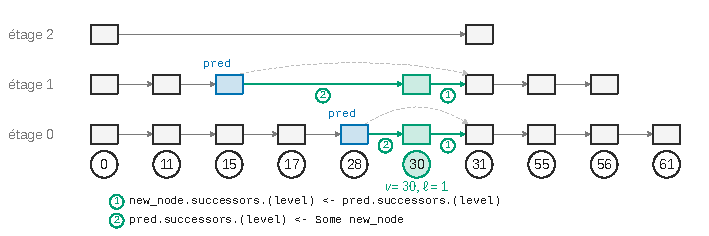
\includegraphics{figures/ii6-insertion-raccordement.pdf}
\caption*{Figure 3 --- Insertion de 30, tiré au niveau 1 : à chaque étage ≤ 1, le
nouveau nœud reprend d'abord le successeur de pred (1), puis pred pointe
vers lui (2)}
\end{figure}

\hypertarget{question-ii.7}{%
\subsection{Question II.7}\label{question-ii.7}}

\textbf{(a)} On suppose que le nœud 0 est présent à l'étage \(L-1\). Sinon, on part de l'étage le plus haut où il est présent.

\begin{lstlisting}[language=Caml]
let closest (query : vector) (g : hgraph) : int =
  let current = ref 0 in
  let level = ref (Array.length g.(0) - 1) in
  let dcur = ref (dist query db.(0)) in
  let fini = ref false in
  while not !fini do
    let best = ref !current and dbest = ref !dcur in
    List.iter (fun j ->
        let dj = dist query db.(j) in
        if dj < !dbest then begin best := j; dbest := dj end)
      g.(!current).(!level);
    if !best <> !current then begin current := !best; dcur := !dbest end
    else if !level = 0 then fini := true
    else level := !level - 1
  done;
  !current
\end{lstlisting}

À chaque tour, on passe au voisin le plus proche de \texttt{query} s'il réduit strictement la distance. Sinon, on descend d'un étage. À l'étage 0, on renvoie le nœud atteint, qui est un minimum local.

\textbf{(b)} On note \(\delta=\texttt{dist query db.(current)}\). Cette quantité décroît strictement à chaque déplacement et ne change pas lors d'une descente. Les nœuds successivement visités sont donc deux à deux distincts, ce qui fait au plus \(n-1\) déplacements. Il y a au plus \(L-1\) descentes. Un même couple (nœud, étage) n'est donc examiné qu'une fois. La liste d'adjacence parcourue au tour courant est celle de ce couple, et l'ensemble des listes parcourues a une longueur totale au plus \(\sum_\ell 2|E_\ell|=2|E|\). Chaque voisin coûte un calcul de distance en \(O(d)\). Complexité :

\equationajustee{\boxed{O\big(d\,(|E|+1)+n+L\big)},}

dominée en pratique par \(O(d\,|E|)\).

\textbf{(c)} \textbf{Non.} La distance \(\delta\) est un variant. Elle décroît strictement à chaque déplacement, donc on ne revient jamais sur un nœud déjà visité. Les déplacements sont en nombre fini, au plus \(n-1\), et les descentes aussi, au plus \(L-1\). L'algorithme termine sans marquage. C'est l'inégalité \emph{stricte} qui garantit cela : avec \(\le\), on pourrait osciller entre deux nœuds équidistants.

\begin{center}\rule{0.5\linewidth}{0.5pt}\end{center}

\hypertarget{partie-iii.-quantification-de-produit}{%
\section{Partie III. Quantification de produit}\label{partie-iii.-quantification-de-produit}}

\hypertarget{question-iii.1}{%
\subsection{Question III.1}\label{question-iii.1}}

\begin{lstlisting}[language=Caml]
let compute_all_dist2 (db : matrix) : square =
  let n = Array.length db in
  Array.init_matrix n n (fun i j -> dist2 db.(i) db.(j))
\end{lstlisting}

Coût : \(n^2\) appels de coût \(O(d)\), soit \(O(n^2 d)\). Par symétrie, on pourrait n'en faire que la moitié.

\hypertarget{question-iii.2}{%
\subsection{Question III.2}\label{question-iii.2}}

Il faut calculer \texttt{dist2\ query\ db.(\allowbreak{}i)\allowbreak{}} pour les \(n\) vecteurs, chacun en \(O(d)\), puis prendre le minimum en \(O(n)\). La complexité est \(\boxed{O(n\,d)}\).

\hypertarget{question-iii.3}{%
\subsection{Question III.3}\label{question-iii.3}}

\begin{lstlisting}[language=Caml]
let pick (db : matrix) (centroids : matrix) (centroid_of : int array) : unit =
  let k = Array.length centroids in
  for i = 0 to Array.length db - 1 do
    let best = ref 0 and dbest = ref (dist2 db.(i) centroids.(0)) in
    for j = 1 to k - 1 do
      let dj = dist2 db.(i) centroids.(j) in
      if dj < !dbest then begin best := j; dbest := dj end
    done;
    centroid_of.(i) <- !best
  done
\end{lstlisting}

On suppose \(k\geq1\). La distance euclidienne et son carré ont le même minimiseur. Coût : \(O(n\,k\,d)\).

\hypertarget{question-iii.4}{%
\subsection{Question III.4}\label{question-iii.4}}

\begin{lstlisting}[language=Caml]
let update (k : int) (db : matrix) (centroid_of : int array)
    (centroids : matrix) : unit =
  let d = Array.length db.(0) in
  let sums = Array.init k (fun _ -> Array.make d 0.) in
  let counts = Array.make k 0 in
  for i = 0 to Array.length db - 1 do
    let j = centroid_of.(i) in
    sums.(j) <- vector_sum sums.(j) db.(i);
    counts.(j) <- counts.(j) + 1
  done;
  for j = 0 to k - 1 do
    if counts.(j) > 0 then
      centroids.(j) <- vector_div sums.(j) (float_of_int counts.(j))
  done
\end{lstlisting}

Le nouveau centroïde \(j\) est la moyenne des vecteurs qui lui sont affectés. Un centroïde dont le groupe est vide est laissé inchangé, ce qui évite une division par 0. Coût : \(O(n\,d+k\,d)\).

\hypertarget{question-iii.5}{%
\subsection{Question III.5}\label{question-iii.5}}

\textbf{Oui.} Le centroïde \(j\) n'est pas mis à jour lorsqu'aucun vecteur ne lui est affecté, c'est-à-dire lorsque \texttt{counts.(j)\ =\ 0}. Exemple : \(db=(0,0,1)\) en dimension 1 et \(k=2\). L'initialisation sur les deux premiers vecteurs donne deux centroïdes égaux à \(0\). \texttt{pick} affecte alors les trois vecteurs au centroïde 0, à cause de l'inégalité stricte (le 1 est à égale distance des deux centroïdes). Le centroïde 1 n'est le plus proche d'aucun vecteur, et un seul centroïde est mis à jour. Plus généralement, un groupe peut se vider au cours des itérations, lorsqu'un centroïde est partout « battu » par d'autres.

Si l'on entend « mis à jour » au sens de « modifié », la réponse reste oui : un centroïde dont le groupe ne change pas d'une itération à l'autre est recalculé à l'identique, ce qui arrive dès que l'algorithme a convergé.

\hypertarget{question-iii.6}{%
\subsection{Question III.6}\label{question-iii.6}}

\begin{lstlisting}[language=Caml]
let kmeans (db : matrix) (k : int) (n_iter : int) : int array * matrix =
  let centroids = Array.init k (fun j -> Array.copy db.(j)) in
  let centroid_of = Array.make (Array.length db) 0 in
  for _ = 1 to n_iter do
    pick db centroids centroid_of;
    update k db centroid_of centroids
  done;
  pick db centroids centroid_of;   (* affectation cohérente avec les centroïdes renvoyés *)
  (centroid_of, centroids)
\end{lstlisting}

Une itération consiste en une affectation (\texttt{pick}) suivie d'un recalcul des centroïdes (\texttt{update}). Le \texttt{pick} final garantit que \texttt{centroid\_of} désigne bien, pour chaque vecteur, le plus proche des centroïdes renvoyés. \texttt{Array.copy} évite que les centroïdes partagent la mémoire des vecteurs de \texttt{db}. Coût : \(O\big((n_{\text{iter}}+1)\,n\,k\,d\big)\).

\hypertarget{question-iii.7}{%
\subsection{Question III.7}\label{question-iii.7}}

\begin{lstlisting}[language=Caml]
(* table des d_l(a, b) pour les centroïdes d'un paquet *)
let table (centroids : matrix) : square =
  let k = Array.length centroids in
  Array.init_matrix k k (fun a b -> dist2 centroids.(a) centroids.(b))

let approx_dist (db : matrix) (k : int) (n_iter : int) (m : int) : square =
  let n = Array.length db in
  let quant =                        (* un couple (codes c_l, table d_l) par paquet *)
    List.map (fun pack -> let (c, cent) = kmeans pack k n_iter in (c, table cent))
      (submatrix db m)
  in
  Array.init_matrix n n (fun i j ->
      List.fold_left (fun acc (c, t) -> acc +. t.(c.(i)).(c.(j))) 0. quant)
\end{lstlisting}

Pour le paquet \(\ell\), \texttt{c.(i)} \(=c_\ell(p_i)\) et \texttt{t.(a).(b)} \(=d_\ell(a,b)\). Le \texttt{fold\_left} calcule donc \(D'_{ij}=\sum_{\ell=1}^m d_\ell\big(c_\ell(p_i),\allowbreak c_\ell(p_j)\big)\).

\begin{figure}[H]
\centering
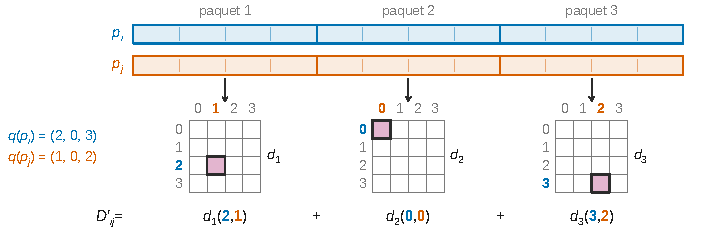
\includegraphics{figures/iii7-quantification-produit.pdf}
\caption*{Figure 4 --- Quantification de produit avec m = 3 paquets et k = 4 : la
distance approchée D′ij est la somme des lectures d1(2, 1), d2(0, 0) et
d3(3, 2) dans les tables des paquets}
\end{figure}

Coût :
- les \(m\) appels aux \(k\)-moyennes sur des vecteurs de dimension \(d/m\) : \(O(n_{\text{iter}}\,n\,k\,d)\) ;
- les tables : \(O(k^2 d)\) ;
- le remplissage de la matrice : \(O(n^2 m)\).

\hypertarget{question-iii.8}{%
\subsection{Question III.8}\label{question-iii.8}}

\textbf{(a)} Le dictionnaire contient une valeur par triplet \((\ell,a,b)\), soit \(m\,k^2\) valeurs. Chacune est le carré d'une distance entre deux centroïdes de dimension \(d/m\), calculé en \(O(d/m)\). Coût total : \(m\,k^2\cdot\frac dm\), soit \(\boxed{O(k^2 d)}\).

\textbf{(b)} \(D'_{ij}\) ne dépend de \((i,j)\) que par le couple de codes

\equationajustee{\big(q(p_i),q(p_j)\big)\in[k]^m\times[k]^m.}

Les \(D'_{ij}\) prennent donc au plus \(\boxed{k^{2m}}\) valeurs distinctes.

On peut affiner. On a \(D'_{ij}=\sum_\ell d_\ell(a_\ell,b_\ell)\), avec \(a_\ell=c_\ell(p_i)\) et \(b_\ell=c_\ell(p_j)\).

Comme \(d_\ell(a,b)=d_\ell(b,a)\), la valeur ne dépend que des \(m\) paires non ordonnées \(\{a_\ell,b_\ell\}\). Il y en a \(\frac{k(k+1)}2\) par paquet, d'où au plus \(\left(\frac{k(k+1)}{2}\right)^m\) valeurs.

Bien sûr, il y a aussi au plus \(n^2\) valeurs.

\textbf{(c)} Les codes de \texttt{db.(i)} et de chaque \texttt{db.(j)} sont stockés. Chaque \(D'_{ij}\) s'obtient par \(m\) lectures dans le dictionnaire et \(m\) additions, soit \(O(m)\).

Pour les \(n\) vecteurs, avec la recherche du minimum, le coût est \(\boxed{O(n\,m)}\). Si l'on veut les voisins triés par distance, il faut ajouter un tri en \(O(n\log n)\).

\textbf{(d)} Il faut d'abord coder le nouveau vecteur \(p\).

Pour chaque paquet \(\ell\), on compare la partie correspondante du vecteur aux \(k\) centroïdes du paquet. Chaque comparaison coûte \(O(d/m)\), donc ce paquet coûte \(O(k\,d/m)\). Sur les \(m\) paquets, le codage coûte \(O(k\,d)\).

On procède ensuite comme en (c), en \(O(n\,m)\). Total : \(\boxed{O(k\,d+n\,m)}\).

C'est à comparer au \(O(n\,d)\) de la recherche exacte (III.2) : le gain est important quand \(n\gg k\) et \(m\ll d\).

\end{document}
